\documentclass{article}
\usepackage{tikz}
\usepackage{amsmath,amsfonts}
\usepackage{caption}
\usepackage{subcaption}
\usepackage{arxiv}
\usetikzlibrary{arrows.meta, bending, positioning}
\usepackage[backend=biber]{biblatex}
\addbibresource{refs.bib}
\usepackage[T1]{fontenc}

\title{Inductive Denoising to Infer Optimal Typology}

\author{Keira Wiechecki}
\date{\today}

\begin{document}

\section{Introduction}

Clustering is denoising is compression is dimension reduction is classification is inference[citation needed].

Compared to unsupervised learning, classifiers for labeled data is a mostly solved problem[citation needed].
This makes converting an unsupervised learning problem to a classification problem a common machine learning approach. RLHF can be seen as one such example. 
Clustering/self-supervision is another, where labels are inferred from the data itself.

Self-supervised classification generally requires substantial ad hoc hyperparameter tuning.
The simplest example is $k$-means clustering, where the number of clusters is directly specified.
Other approaches can find an optimal number of clusters by first constructing intermediate graph representation of the data.
This graph can be partitioned into clusters that maximize modularity\cite{PhysRevE.74.016110}, which is defined as 
\begin{equation}
 \mathcal{H} = \frac{1}{2m}\sum_{c}( \,e_c - \gamma\frac{K_c^2}{2m}) \, 
\end{equation}
where $m$ is the average degree of the graph, $e_c$ is the number of edges in cluster $c$, and $K_c$ is the number of nodes in cluster $c$.
This equation has a nicely intuitive interpretation. Modularity $\mathcal{H}$ of a graph is given by the sum of how well-connected its clusters are,
defined as the difference between the number of edges in the cluster and the expected number of edges given the number of nodes in the graph and average degree of a node.

Although optimizing modularity is NP-hard, it can be approximated using the leiden algorithm\cite{traag2019louvain}.

Though modularity ensures that clusters are well-connected, the number of clusters returned is dependent on $\gamma$, which cannot be inferred from the data. A value of $k$ must also be selected for the input graph.

Clustering can be thought of as a form of denoising. Clusters represent the underlying ``signal'' of a data set. Variation within clusters is ``noise''.

We define a \textit{typology} as an injective mapping of a random vector to a set of \textit{informative central cases}.% plus a random variable. We refer to the random variable as \textit{epiphenomena}.
%As opposed to noise, epiphenomena may encode information, but it is ``out of scope''.
We define an \textit{ontology} as a function that encodes a random vector $\mathbf{x}$ as a composition of typologies applied to $\mathbf{x}$.
Look at
Let $\Omega$ be an ontology of data $X$ consisting of $n$ typologies.
Let $\Theta$ be a typology in $\Omega$ and $\mathbf{\hat{x}}$ be an encoding of a vector $\mathbf{x} \in X$.
Let $\Theta_0(\mathbf{x}) = \mathbf{0}$.
\begin{equation}
  \Omega(\mathbf{x}) = \bigoplus_{i=1}^{n}\Theta_i(\mathbf{x} - \Theta_{i-1}(\mathbf{x}))
\end{equation}
We propose that by minimizing the self-supervised loss function
\begin{equation}
  \mathcal{L}(\Omega) = \mathbb{E}||\mathrm{sum}[\Omega(\mathbf{x})] - \mathbf{x}||^2
\end{equation}
we can obtain a maximally informative ontology.

\subsection{DEWAK*}
Noise2self\cite{batson2019} applies self-supervision to denoising.
DEWAKSS\cite{tjarnberg2021} uses noise2self selects optimal hyperparameters for generating a $k$-NN represeantation of single cell RNA-seq by using an arbitrary graph as a weighted affinity kernel

Let $\mathcal{G}$ be a set of graphs generated from data $X$ using a variable hyperparameter $h$.
Let $G_\phi \in \mathcal{G}$ be an adjacency matrix for the graph generated by $h := \phi$ normalized to be a right stochastic matrix.
For each graph we can obtain an estimator for data $X$
\begin{equation}
  \hat{X}_\phi = G_\phiX
\end{equation}
and minimize the loss function
\begin{equation}
  \mathcal{L}(\hat{X}_\phi) = (X - \hat{X}_\phi)^2
\end{equation}
to obtain an optimal $\phi$.

We define a typology $\Theta$ as a partition $\mathcal{J}$ of data $X$ such that each subset $J \in \mathcal{J}$ is associated with a central member $\hat{x}_J \in \hat{X}_\mathcal{J}$.
$\hat{X}_\mathcal{J}$ is given by applying an estimator $\underset{J \in \mathcal{J}}{\bigoplus}\mathbb{E}[J]$

\section{Methods}

\subsection{Dimension Reduction}

Many parameters are strongly correlated (Fig. 2b). This is undesirable because each parameter additively contributes to distance used for clustering, resulting in disproportionate weight being given to phenotypes captured by multiple parameters. Linear methods of dimenison reduction (e.g. PCA) assume that all variables are independent and can be linearly combined. We could not assume that all of our measured input parameters were independent, so we instead used an autoencoder for dimension reduction.

An autoencoder is a neural network architecture widely used for denoising and image recognition. It works by encoding the input data into a lower dimensional representation that can be decoded with minimal loss. By extracting this lower dimensional encoding (the ``bottleneck'' or ``embedding'' layer), an autoencoder can be used for dimension reduction\cite{WANG2016232}. This results in an embedding that corresponds to the information content of the input data rather than absolute distance in phenotype space.

\subsubsection{Pruning}

We trained four autoencoders using embedding layers of 2, 3, 7, and 14 dimensions. We selected the 2-dimensional embedding based on Akaike Information Criterion\cite{cavanaugh2019akaike} (Table 1; Fig. 1a), defined as 
\begin{equation}
AIC = 2k - 2ln(\hat{L}) 
\end{equation}
where $k$ is the number of parameters and $\hat{L}$ is a likelihood function, which we define as $1 - MSE$.

\subsection{Clustering Algorithm}
Euclidean distance between embeddings is used to compute a k-nearest neighbors graph. The graph is then partitioned into clusters by modularity\cite{PhysRevE.74.016110}, which is defined as 
\begin{equation}
 \mathcal{H} = \frac{1}{2m}\sum_{c}( \,e_c - \gamma\frac{K_c^2}{2m}) \, 
\end{equation}
 where $m$ is the average degree of the graph, $e_c$ is the number of edges in cluster $c$, and $K_c$ is the number of nodes in cluster $c$. This equation has a nicely intuitive interpretation. Modularity $\mathcal{H}$ of a graph is given by the sum of how well-connected its clusters are, defined as the difference between the number of edges in the cluster and the expected number of edges given the number of nodes in the graph and average degree of a node.

Because optimizing modularity is NP-hard, we used the leiden algorithm to approximate an optimal solution\cite{traag2019louvain}.

Though modularity ensures that clusters are well-connected, the number of clusters returned is dependent on $\gamma$, which cannot be inferred from the data. A value of $k$ must also be selected for the input graph.

\subsection{Hyperparameter Selection}

We performed clustering for 100 random $\gamma$ values between 0.01 and 3.0 for $k$ values ranging from 3 to 53.

We selected $k$ and $\gamma$ based on four validation metrics. Mean silhouette width was calculated from the euclidean distance etween embryos.

\subsubsection{$k$ Selection}
\begin{figure}
    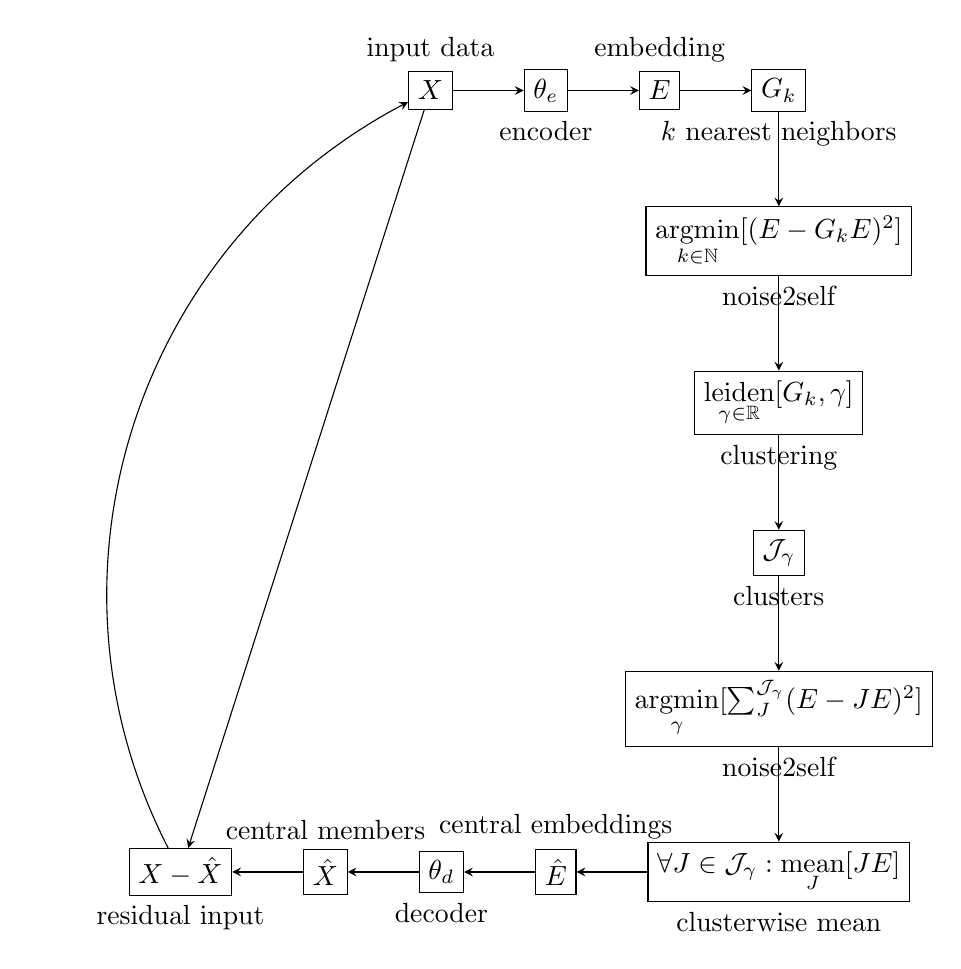
\begin{tikzpicture}[
node distance = 12mm and 9mm,
 punkt/.style = {rectangle, draw},
   pil/.style = {black, -stealth}
                    ]
%nodes
\node[punkt,label=above:input data] (X)                                  {$X$} ;
\node[punkt,label=below:encoder] (encoder) [right=of X] {$\theta_e$} ;
\node[punkt,label=above:embedding] (E) [right=of encoder] {$E$} ;
%\node (noise2self) [below=of E] {$\mathrm{noise2self}$} ;

%\node (knn) [right=of E] {$k$ nearest neighbors};
\node[punkt,label=below:$k$ nearest neighbors] (G) [right=of E] {$G_k$};
\node[punkt,label=below:noise2self] (ksel) [below=of G] {$\underset{k \in \mathbb{N}}{\mathrm{argmin}} [(E - G_kE)^2]$};
\node[punkt,label=below:clustering] (leiden) [below=of ksel] {$\underset{\gamma \in \mathbb{R}}{\mathrm{leiden}} [G_k,\gamma]$};
\node[punkt,label=below:clusters] (J) [below=of leiden] {$\mathcal{J}_\gamma$};
\node[punkt,label=below:noise2self] (gammasel) [below=of J] {$\underset{\gamma}{\mathrm{argmin}} [\sum_J^{\mathcal{J}_{\gamma}}(E - JE)^2]$};
\node[punkt,label=below:clusterwise mean] (mean) [below=of gammasel] {$\forall J \in \mathcal{J}_\gamma : \underset{J}{\mathrm{mean}}[JE]$};

\node[punkt,label=above:central embeddings] (Ehat) [left=of mean] {$\hat{E}$} ;
\node[punkt,label=below:decoder] (decoder) [left=of Ehat] {$\theta_d$} ;
\node[punkt,label=above:central members] (Xhat) [left=of decoder] {$\hat{X}$} ;
\node[punkt,label=below:residual input] (resid) [left=of Xhat] {$X - \hat{X}$} ;

% edges
\draw[pil]  (X)     edge    (encoder)
(encoder) edge (E)
%(E) edge (noise2self)
%(noise2self) edge (Ehat)
(Ehat) edge (decoder)
(decoder) edge (Xhat)
(Xhat) edge (resid)
(X)    edge    (resid)
(resid) edge[bend left=45] (X) ;


\draw[pil] (E) edge (G)
%(knn) edge (G)
(G) edge (ksel)
(ksel) edge (leiden)
(leiden) edge (J)
(J) edge (gammasel)
(gammasel) edge (mean)
(mean) edge (Ehat);
    \end{tikzpicture}
    \caption{Typology block.}
    \label{fig:}
    \end{figure}

\printbibliography
\end{document}
